%	This is written by Zhiyang Ong as a template for writing reports.

%	The MIT License (MIT)

%	Copyright (c) <2014> <Zhiyang Ong>

%	Permission is hereby granted, free of charge, to any person obtaining a copy of this software and associated documentation files (the "Software"), to deal in the Software without restriction, including without limitation the rights to use, copy, modify, merge, publish, distribute, sublicense, and/or sell copies of the Software, and to permit persons to whom the Software is furnished to do so, subject to the following conditions:

%	The above copyright notice and this permission notice shall be included in all copies or substantial portions of the Software.

%	THE SOFTWARE IS PROVIDED "AS IS", WITHOUT WARRANTY OF ANY KIND, EXPRESS OR IMPLIED, INCLUDING BUT NOT LIMITED TO THE WARRANTIES OF MERCHANTABILITY, FITNESS FOR A PARTICULAR PURPOSE AND NONINFRINGEMENT. IN NO EVENT SHALL THE AUTHORS OR COPYRIGHT HOLDERS BE LIABLE FOR ANY CLAIM, DAMAGES OR OTHER LIABILITY, WHETHER IN AN ACTION OF CONTRACT, TORT OR OTHERWISE, ARISING FROM, OUT OF OR IN CONNECTION WITH THE SOFTWARE OR THE USE OR OTHER DEALINGS IN THE SOFTWARE.

%	Email address: echo "cukj -wb- 23wU4X5M589 TROJANS cqkH wiuz2y 0f Mw Stanford" | awk '{ sub("23wU4X5M589","F.d_c_b. ") sub("Stanford","d0mA1n"); print $5, $2, $8; for (i=1; i<=1; i++) print "6\b"; print $9, $7, $6 }' | sed y/kqcbuHwM62z/gnotrzadqmC/ | tr 'q' ' ' | tr -d [:cntrl:] | tr -d 'ir' | tr y "\n"

%%%%%%%%%%%%%%%%%%%%%%%%%%%%%%%%%%%%%%%%%%%%%%


%%%%%%%%%%%%%%%%%%%%%%%%%%%%%%%%%%%%%%%%%%%
\section{Superscalar Processor Design}
\label{sec:SuperscalarProcessorDesign}


%    Hennessy2012
%    Chapter 3, 
%    
%    Hennessy2007
%    Chapter 2, 3,
%    
%    Hennessy2003
%    Chapter 3,

To improve the performance of pipelined processors, multiple instructions can be issued at the same time (i.e., superscalar instruction issue) in the pipelined microarchitecture; scalar processors can only issue one instruction per clock cycle. Therefore, superscalar processors allow the throughput of instruction execution to increase by exploiting instruction-level parallelism via instruction scheduling, loop unrolling, and branch prediction to reduce unnecessary stalls in the pipelined datapath \cite{Hennessy2012,Shen2005a}. However, the scope of literature on techniques to improve the performance of superscalar processors, including superpipelined and superscalar processors, is vast. Hence, I would only briefly mention the important concepts behind superscalar processors. \\



\begin{figure}[h]
\centering 
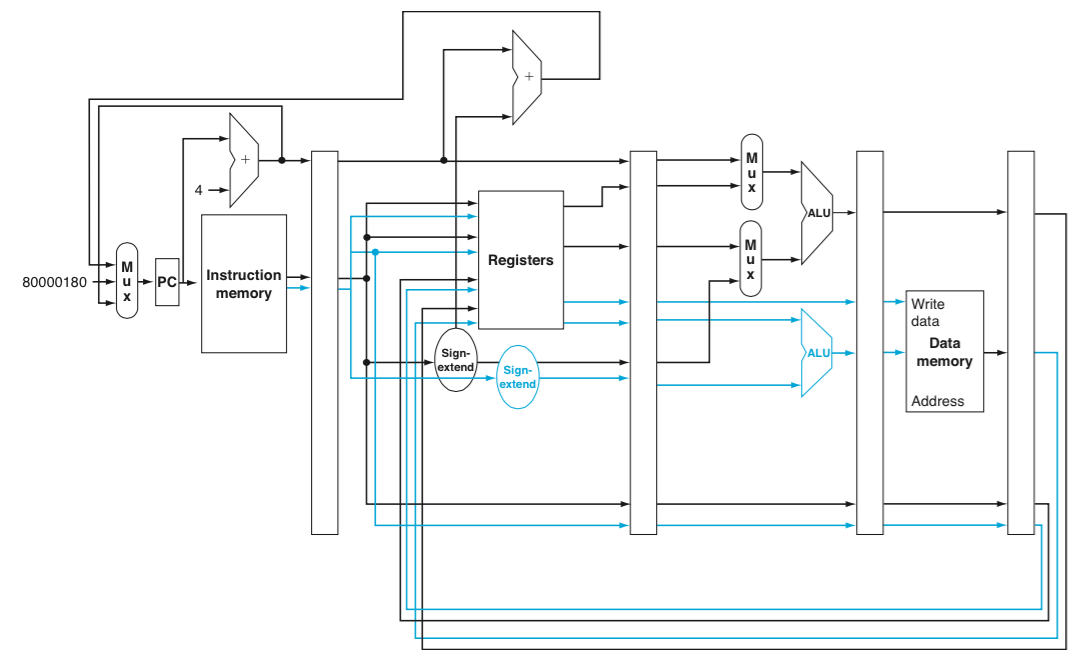
\includegraphics[width=6in]{./pics/superscalar-static-pipeline}
\caption{The static datapath pipeline of a superscalar processor \cite{Patterson2012}.}
\label{fig:superscalarstaticpipeline}
\end{figure}

\begin{figure}[h]
\centering 
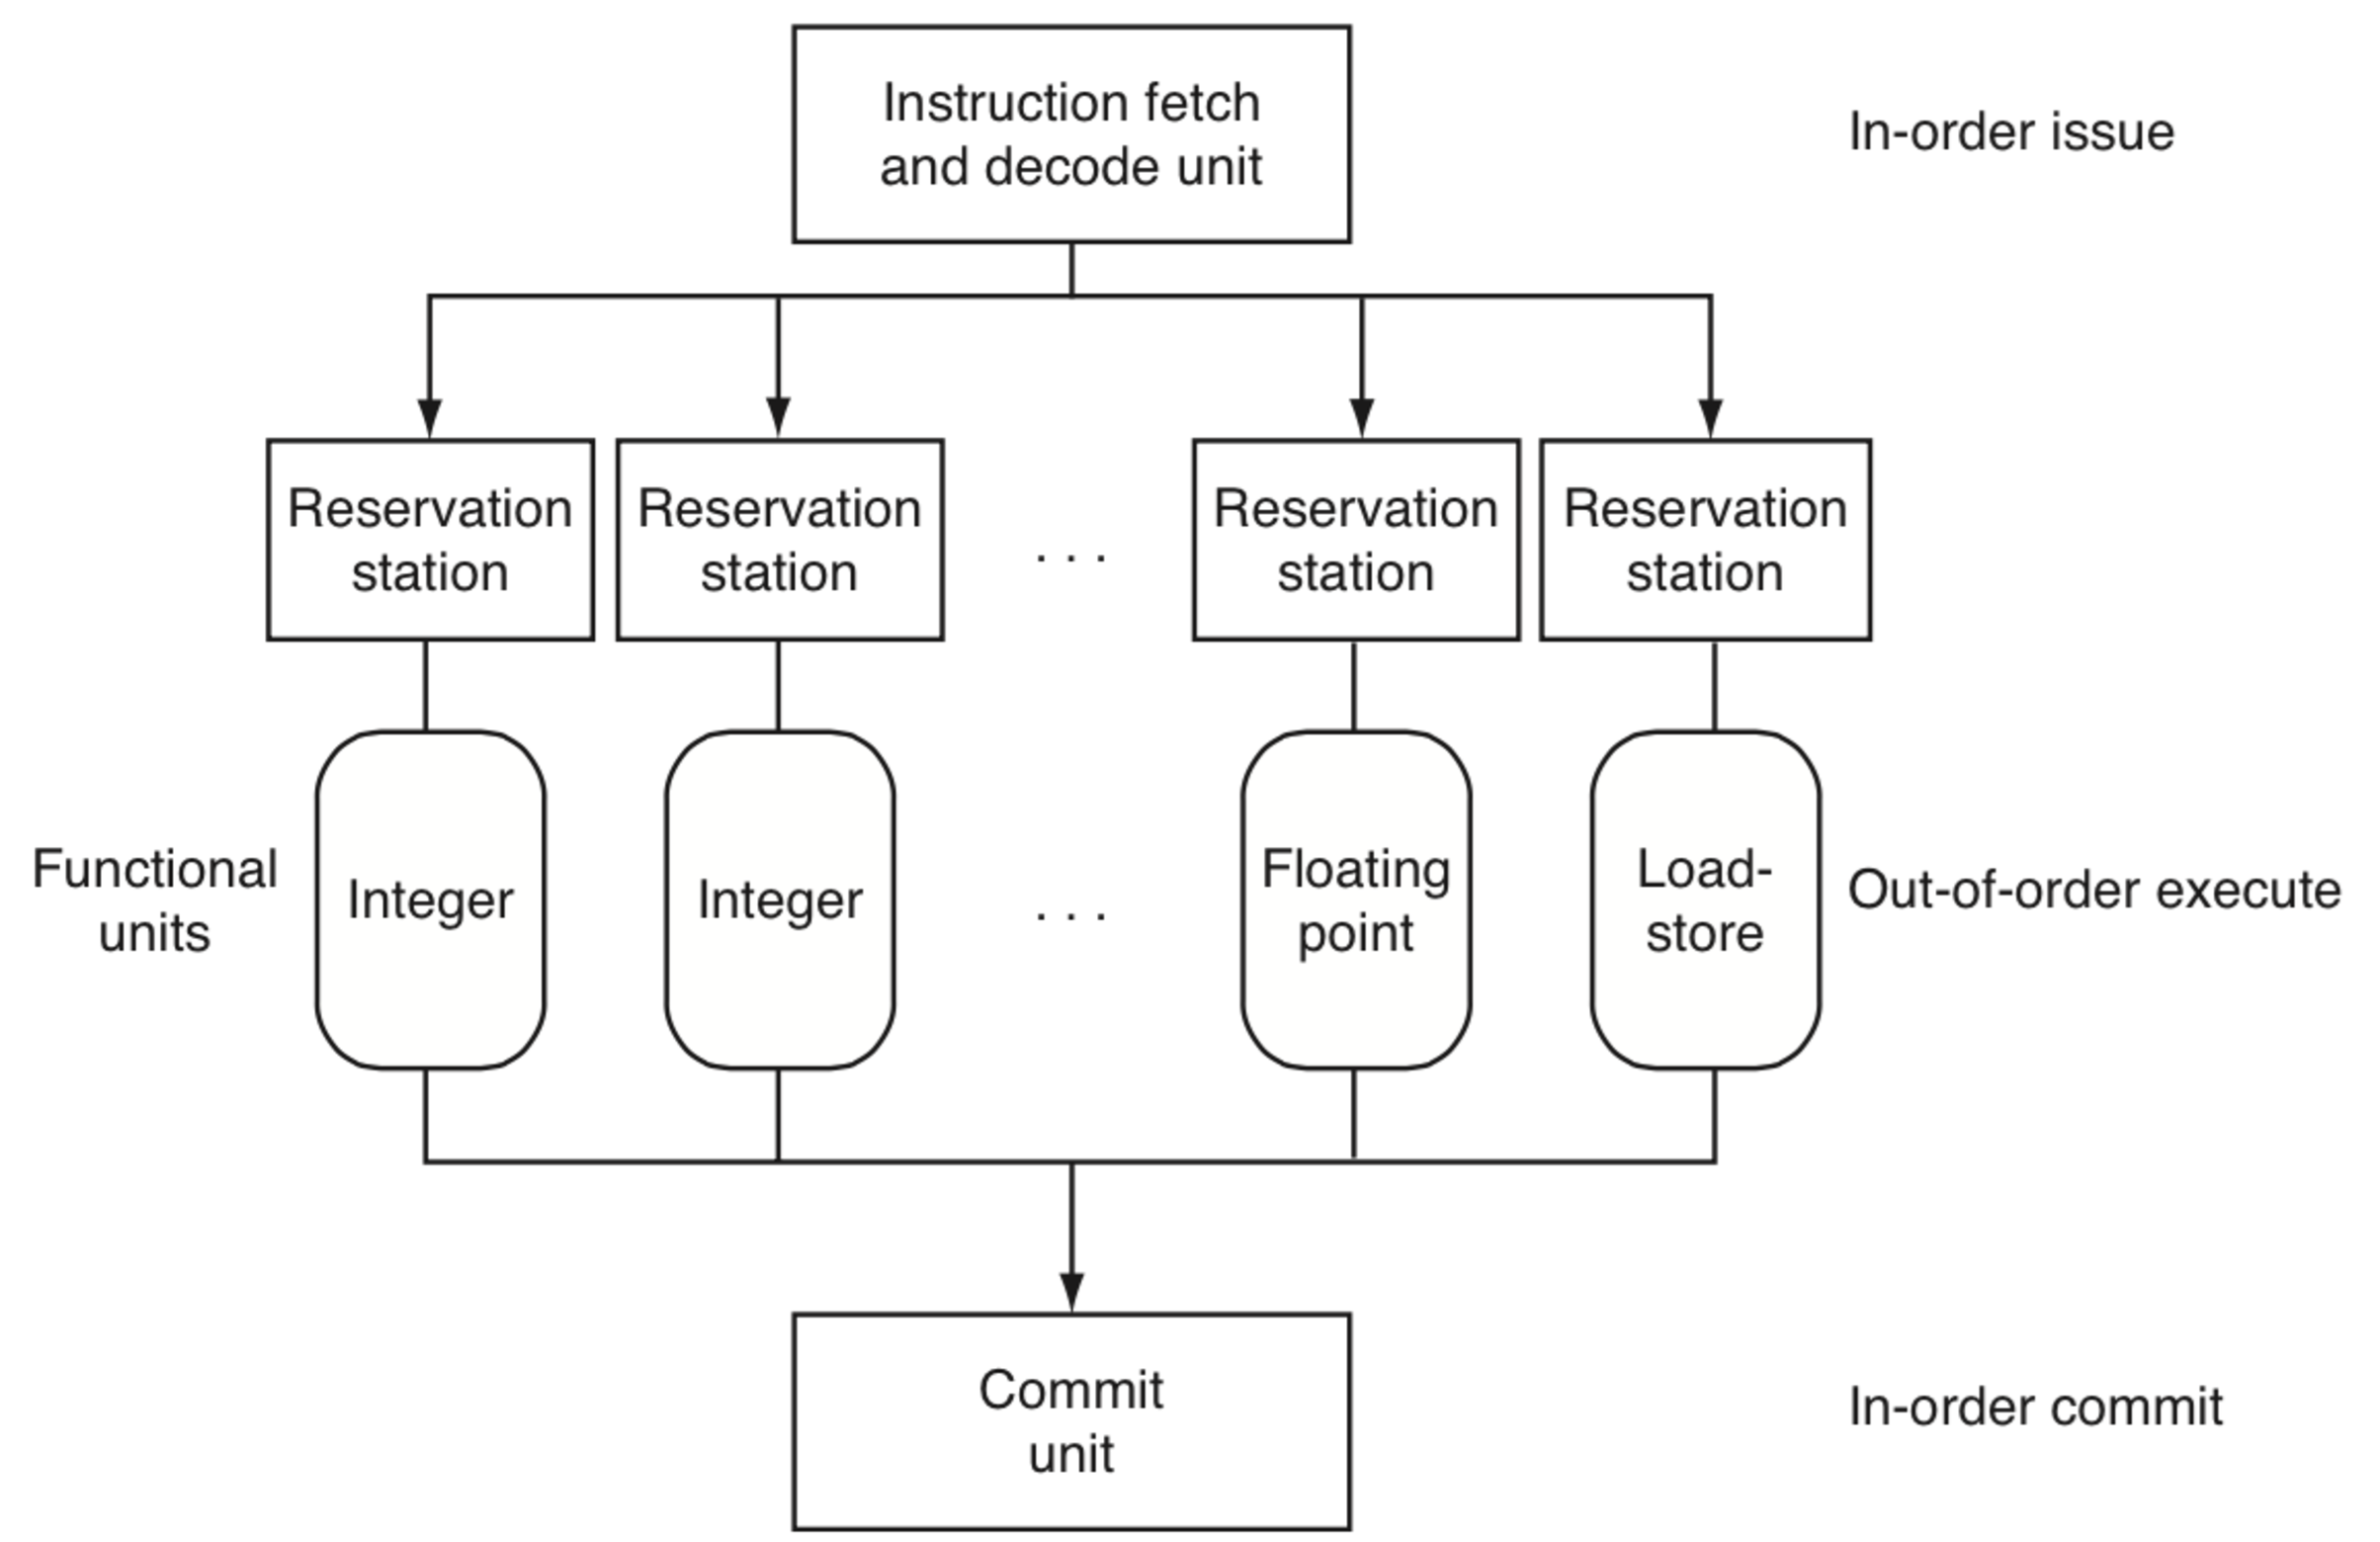
\includegraphics[width=6in]{./pics/superscalar-dynamic-pipeline}
\caption{The dynamic datapath pipeline of a superscalar processor \cite{Patterson2012}.}
\label{fig:superscalardynamicpipeline}
\end{figure}

%    static two-issue datapath 
%    Figure 6.45, Patterson2005, pp. 437
%    Figure 4.69, Patterson2012, pp. 395

%    Datapath of dynamically scheduled pipeline of $n$-issue superscalar processors
%    Figure 6.49, Patterson2005, pp. 444
%    Figure 4.72, Patterson2012, pp. 399


%    Pentium 4 datapath 
%    Figure 6.50, Patterson2005, pp. 449
%    AMD Opteron X4 microarchitecture
%    Figure 4.74, Patterson2012, pp. 405


\begin{figure}[h]
\centering 
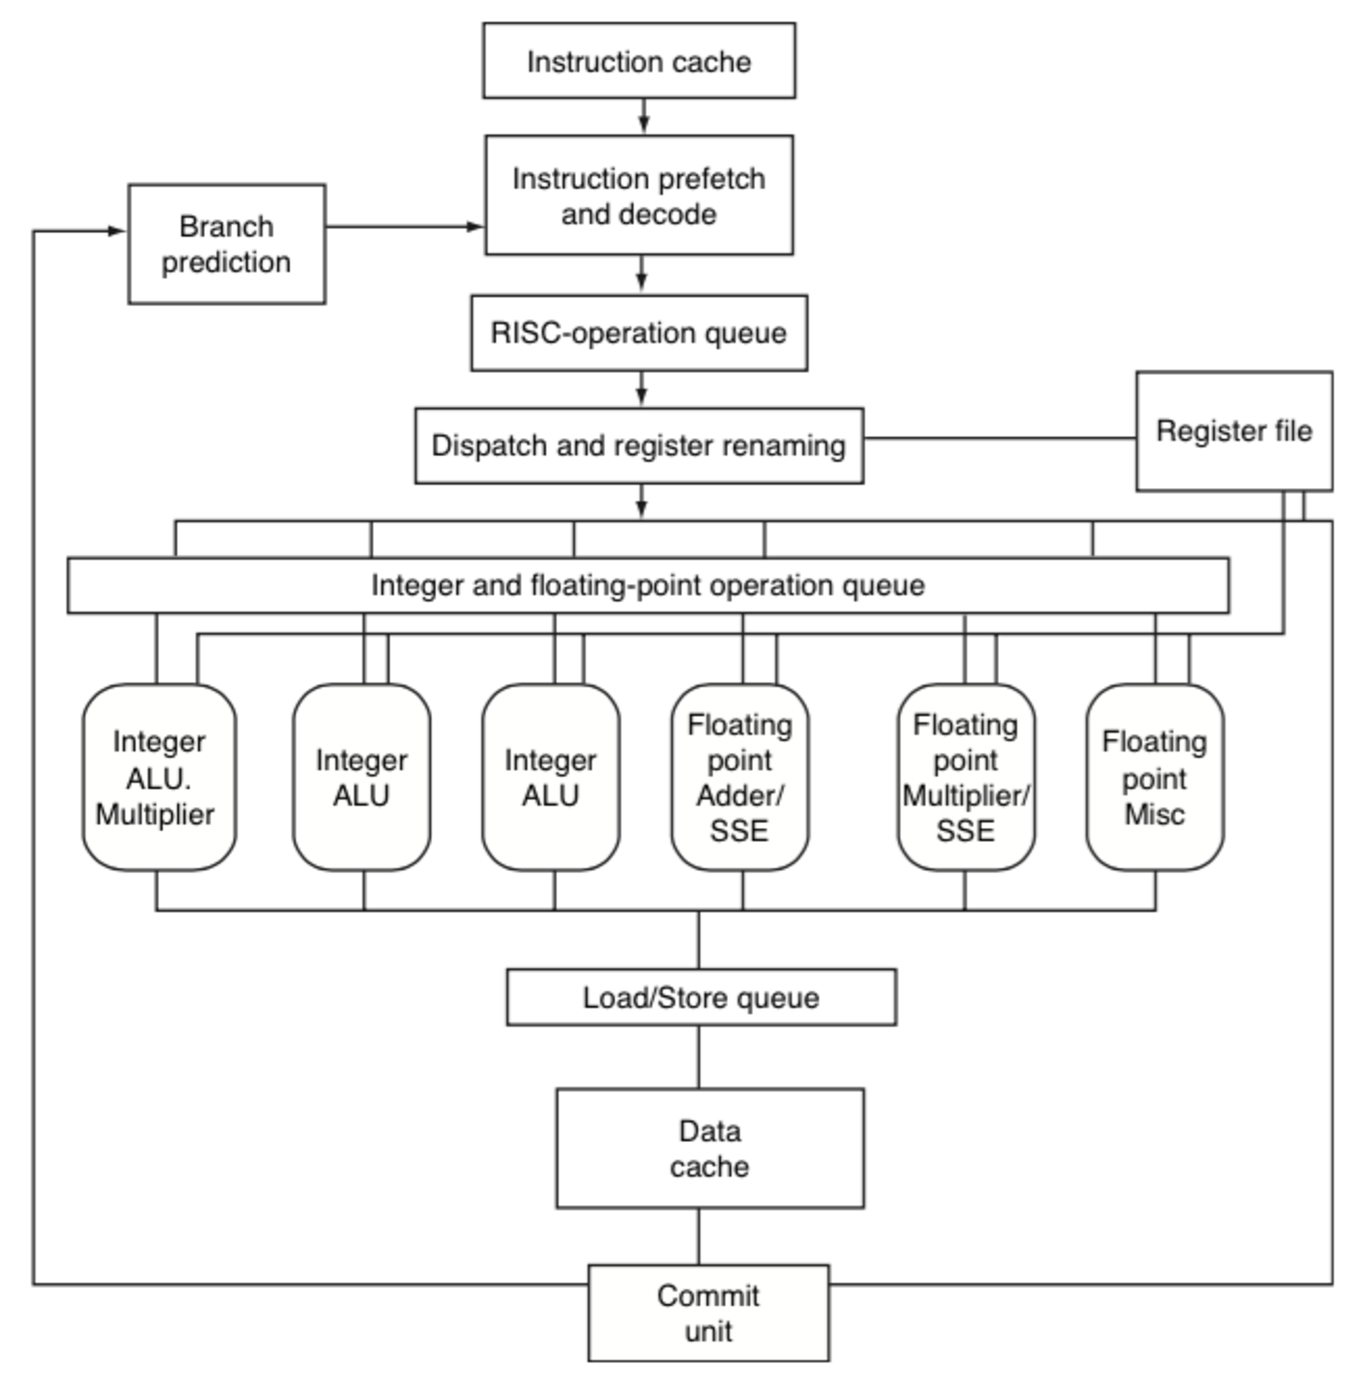
\includegraphics[width=6in]{./pics/amd-opteron-x4-uarch}
\caption{Dynamic pipelined datapath of the AMD Opteron X4 processor's microarchitecture \cite{Patterson2012}.}
\label{fig:amdopteronx4uarch}
\end{figure}

A brief description of static and dynamic pipelined, superscalar processors is provided as follows. Figure \ref{fig:superscalarstaticpipeline} shows the static datapath pipeline of a superscalar processor \cite{Patterson2012}. It issues multiple instructions per clock cycle, and has two separate datapath pipelines of functional units to support superscalar execution of instructions. In Figure \ref{fig:superscalardynamicpipeline}, a dynamic datapath pipeline of a superscalar processor is shown \cite{Patterson2012}; such superscalar processors are also known as out-of-order, superscalar processors. Instruction scheduling and loop unrolling are exploited to allow instructions to be issued in order, executed out of order (due to instruction scheduling), and completed in order so that less bubbles have to be issued in the datapath pipeline. Here, loop unrolling increases the window size of instructions that the compiler or corresponding hardware can use to carry out instruction scheduling. In order for dynamic pipelined, superscalar processors to function correctly, reservation stations (or a dispatch buffer) is placed between the front-end of the processor (for instruction fetch and decode) and the execution stage. They ensure that instructions are issued in order as they appear in the instruction stream. In addition, reorder buffers in the commit unit must be used to complete and retire the executed instructions in order. This in-order retirement of instructions guarantees the functional correctness of running computer programs on that out-of-order superscalar processor
\cite{Hennessy2012,Shen2005a}. Figure \ref{fig:amdopteronx4uarch} shows the dynamic pipelined datapath of the AMD Opteron X4 processor's microarchitecture \cite{Patterson2012}. It reflects multi-instruction issue in contemporary microarchitectures and the use of parallel functional units to support superscalar instruction issue, such as three integer ALUs in this example.


























































